%%%%%%%%%%%%%%%%%%%%%%%%%%%%%%%%%%%%%%%%%%%%%%%%%%%%%%%%%%%%%%%%%%%%%%
%     File: ExtendedAbstract_imple.tex                               %
%     Tex Master: ExtendedAbstract.tex                               %
%%%%%%%%%%%%%%%%%%%%%%%%%%%%%%%%%%%%%%%%%%%%%%%%%%%%%%%%%%%%%%%%%%%%%%

\section{Aerial-D Dataset Construction}
\label{sec:approach}

\subsection{Source Datasets}

The AerialD dataset is constructed from two primary sources of aerial imagery with fundamentally different annotation paradigms. The iSAID dataset provides instance segmentation annotations with 655,451 instances across 15 object categories including ships, vehicles, planes, buildings, and infrastructure elements such as harbors and bridges. The dataset contains 2,806 high-resolution aerial images with varying dimensions and spatial resolutions ranging from 0.1m to 4.5m per pixel. In contrast, the LoveDA dataset offers semantic segmentation annotations capturing land cover patterns across 5,987 images at 1024×1024 resolution with 0.3m spatial resolution. It provides pixel-level classification into six categories: buildings, roads, water bodies, agricultural areas, forests, and barren land.

These complementary datasets ensure comprehensive coverage of both discrete objects and continuous landscape features commonly encountered in aerial imagery analysis. The combination enables our pipeline to generate referring expressions for individual object instances from iSAID while also supporting semantic region descriptions from LoveDA's land cover classifications.

\subsection{Rule-Based Expression Generation}

In order to generate referring expressions for objects annotated in the source datasets, we must first extract manageable patches from the high-resolution aerial images. Since iSAID contains images with varying dimensions up to 13,000 pixels, we employ a sliding window approach with 480×480 patches and overlap to ensure all instances are captured with sufficient context. We also group instances using DBSCAN clustering early in the process and create category-level segmentations, then apply spatial and visual rules that map into particular referring expressions.

To provide spatial context for object localization, we utilize bounding box coordinates to analyze centroids and determine which region of the image objects occupy. As shown in Figure \ref{fig:rule_example}, the system divides each patch into a three-by-three grid with dotted lines, creating nine distinct spatial regions such as "top left", "center", and "bottom right". We also identify instances that occupy extreme positions (topmost, bottommost, leftmost, rightmost) within their respective categories when multiple objects of the same type are present.

In order to provide visual characteristics that can distinguish between similar objects, we analyze HSV pixel values within each instance mask to determine color properties. The classification process distinguishes between achromatic colors (light and dark) and chromatic colors across distinct hues. We filter out color references for buildings and water instances, as these objects typically exhibit multi-hue patterns that do not provide meaningful discriminative information.

To enable complex referring expressions, we implement spatial relationship calculation between object pairs using an angle-based directional system across eight directions: to the left of, to the bottom left of, below, to the bottom right of, to the right of, to the top right of, above, and to the top left of. This addresses cases where absolute grid positions alone cannot uniquely identify objects.

Having extracted all spatial, visual, and relational attributes, the system synthesizes these components into referring expressions through combinatorial templates, as demonstrated in Figure \ref{fig:rule_example}. However, the fundamental challenge emerges when multiple objects possess identical attributes, inevitably generating expressions that are exactly the same and creating ambiguous references. To resolve this critical issue, we implement uniqueness filtering that systematically identifies and removes all expressions that appear multiple times across the dataset, ensuring every remaining phrase uniquely identifies a single object or group. Objects that lose all their expressions during this filtering process are eliminated entirely from the dataset.

\begin{figure*}[t]
\centering
\begin{minipage}{0.5\textwidth}
\centering
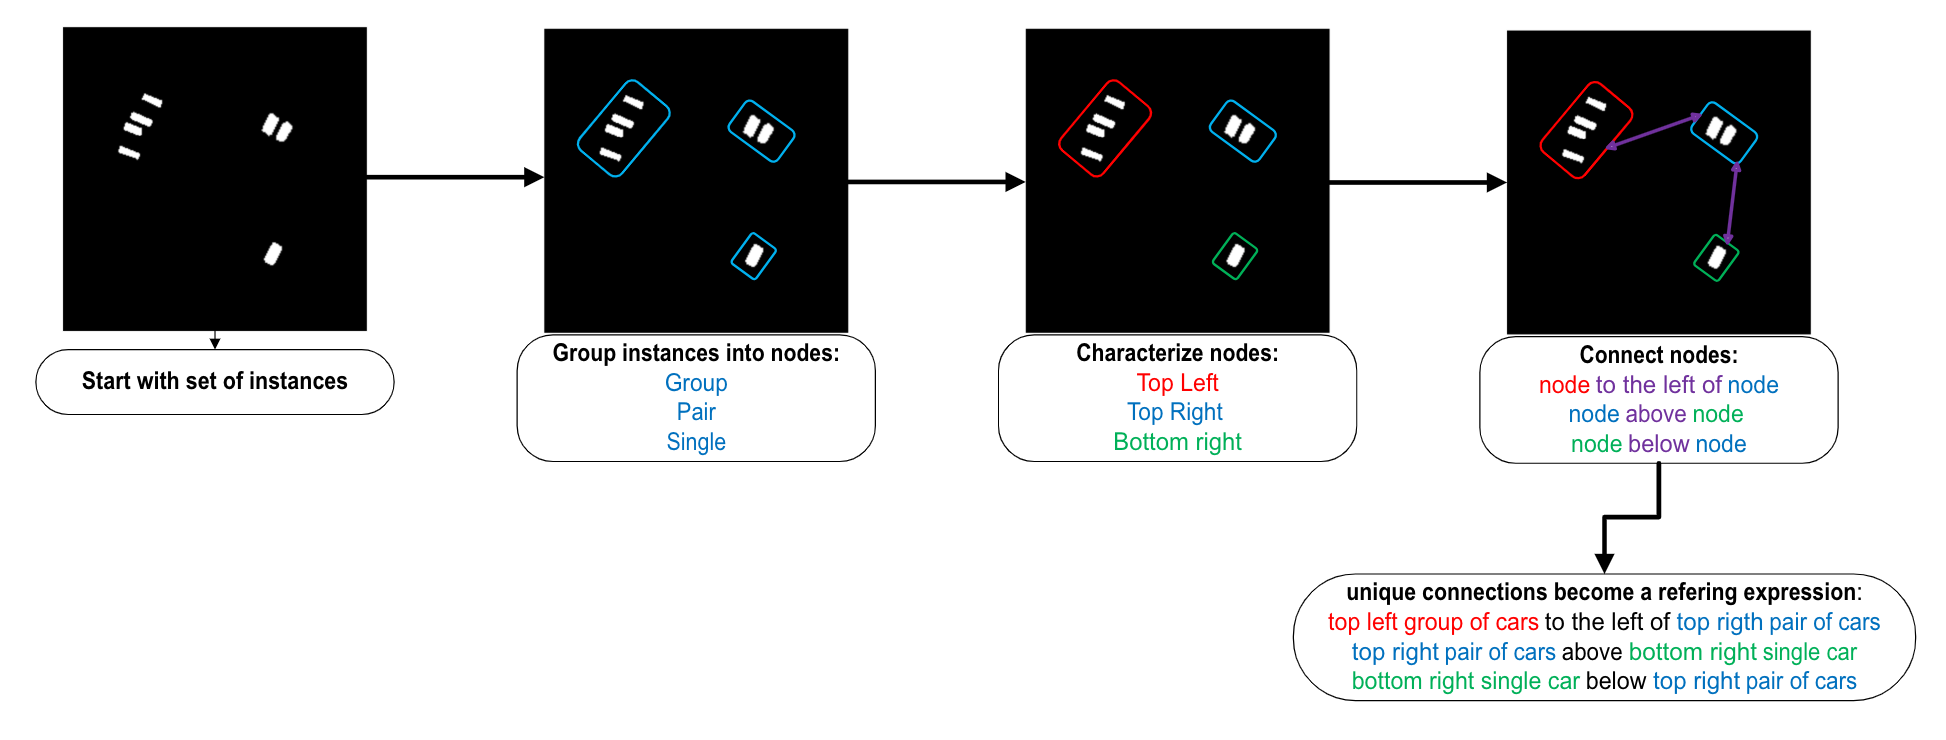
\includegraphics[width=0.7\textwidth]{./images/rule_based_generation.png}
\end{minipage}%
\begin{minipage}{0.5\textwidth}
\centering
\hspace{-1cm}
\raisebox{-0.3\height}{%
\resizebox{\textwidth}{!}{%
\footnotesize
\begin{tabular}{@{}ll@{}}
\toprule
\textbf{Rule Type} & \textbf{Example Instance} \\
\midrule
Category & "plane" \\
Grid Position & "in the top right" \\
Extreme Position & None \\
Color Classification & "light" \\
Directional Relations & "to the bottom right of a plane" \\
& "to the top right of a plane" \\
\midrule
\multicolumn{2}{l}{\textbf{Final Expressions}} \\
\multicolumn{2}{l}{"the plane in the top right"} \\
\multicolumn{2}{l}{"the light plane in the top right"} \\
\multicolumn{2}{l}{"the plane in the top right to the bottom right of a plane"} \\
\multicolumn{2}{l}{"the light plane in the top right to the bottom right of a plane"} \\
\multicolumn{2}{l}{"the plane in the top right to the top right of a plane"} \\
\multicolumn{2}{l}{"the light plane in the top right to the top right of a plane"} \\
\bottomrule
\end{tabular}%
}%
}
\end{minipage}
\caption{Example of rule generation for a single instance. The highlighted plane in the top right section demonstrates how the system assigns spatial, visual, and relational rules that will later be combined into referring expressions.}
\label{fig:rule_example}
\end{figure*}


\subsection{LLM Expression Generation}

While rule-based expression generation provides a solid foundation for referring expression data, these expressions suffer from significant limitations in language variation and visual detail coverage. The rule-based approach produces linguistically constrained expressions with limited wording variations and lacks the ability to reference contextual elements beyond predefined source dataset categories.

To address these limitations, we employ large language models to enhance our dataset through two primary mechanisms: language enhancement to diversify linguistic patterns beyond simple templates, and visual enhancement to incorporate detailed descriptions of contextual objects not captured in the original datasets. As demonstrated in Figure \ref{fig:llm_enhancement_example}, the LLM enhancement process transforms basic expressions like "the group of 4 large vehicles in the top center" into linguistically diverse alternatives such as "the cluster of four big vehicles near the upper middle" and visually detailed descriptions like "the four large vehicles lined up side by side just below the pale paved strip at the very top middle".

However, applying production-grade models directly to our massive dataset presents significant computational and financial challenges. Processing 300,000 targets through premium APIs would be prohibitively expensive for research-scale dataset construction.

To address this scalability challenge, we implement knowledge distillation that transfers the capabilities of large proprietary models to smaller, open-source alternatives. Our distillation pipeline begins by processing a carefully selected subset of 500 objects through OpenAI's o3 model to generate optimal expression enhancements. These high-quality outputs serve as training targets for fine-tuning Gemma3-12B using QLora techniques.

The fine-tuned Gemma3 model can then be deployed locally using vLLM inference on a single GPU to process the entire dataset, generating millions of enhanced expressions. This approach transforms what would have been a costly process requiring premium API access into a manageable operation on standard GPU hardware while maintaining enhancement quality comparable to the original o3 outputs.

\begin{figure*}[t]
\centering
\begin{minipage}{0.5\textwidth}
\centering
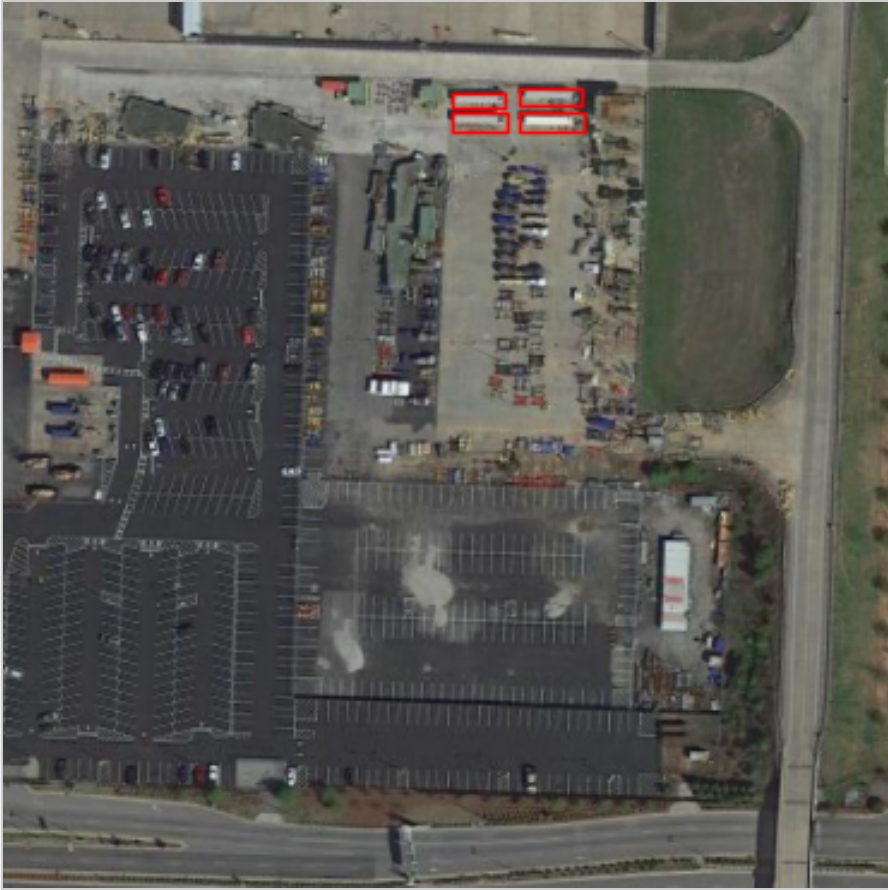
\includegraphics[width=0.7\textwidth]{./images/example_group.png}
\end{minipage}%
\begin{minipage}{0.5\textwidth}
\centering
\hspace{-1cm}
\raisebox{-0.3\height}{%
\footnotesize
\begin{tabular}{@{}p{2cm}p{5cm}@{}}
\toprule
\textbf{Expression Type} & \textbf{Example} \\
\midrule
Original & the group of 4 large vehicles in the top center \\
\midrule
Enhanced & the cluster of four big vehicles near the upper middle \\
\midrule
Unique & the four large vehicles lined up side by side just below the pale paved strip at the very top middle \\
\midrule
Unique & the set of four big vehicles parked in a single row in the upper center beside the grassy area to the right \\
\bottomrule
\end{tabular}%
}
\end{minipage}
\caption{Example of LLM enhancement process showing original aerial image with group of four large vehicles (left) and corresponding expression enhancements (right).}
\label{fig:llm_enhancement_example}
\end{figure*}


\begin{figure}[H]
\centering
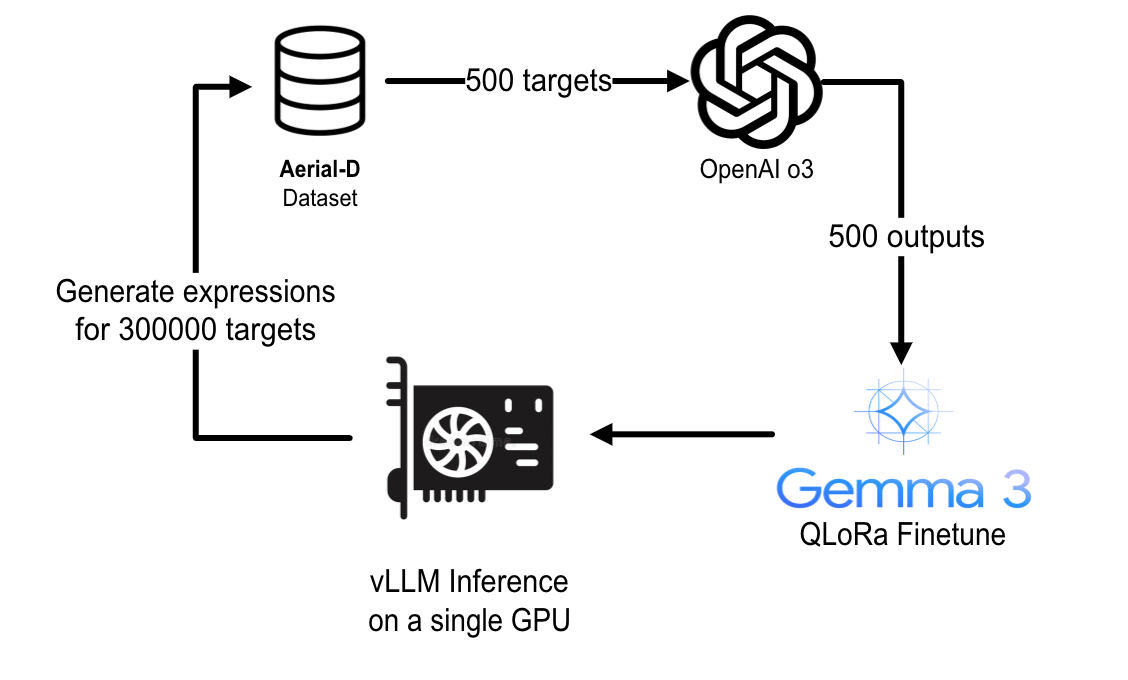
\includegraphics[width=0.8\columnwidth]{./images/distillation.png}
\caption{Knowledge distillation pipeline for scalable LLM enhancement. A small sample of 500 expressions is processed through OpenAI's O3 model to generate high-quality training targets, which are then used to fine-tune Gemma3 12B via QLora. The fine-tuned model enables cost-effective local inference to enhance the full dataset of 300,000 expressions using vLLM on a single GPU.}
\label{fig:llm_distillation}
\end{figure}

\subsection{Final Dataset Statistics}

The completed AerialD dataset represents a comprehensive resource for aerial referring expression segmentation, containing over 1.5 million expressions across diverse object categories and linguistic patterns. The dataset achieves substantial scale with 37,288 total patches containing 259,709 annotated samples, maintaining balanced distribution between individual objects (128,715 instances with 889,354 expressions) and groups (130,994 groups with 633,169 expressions).

The dataset encompasses both discrete objects from iSAID and semantic land cover categories from LoveDA, ensuring comprehensive representation of aerial imagery content. Small vehicles represent the most abundant category with 41,353 individual instances, while specialized categories like helicopters and baseball diamonds provide targeted coverage for specific aerial object types.

The systematic generation pipeline produces expressions through seventeen distinct templates, ranging from simple category references to complex multi-attribute descriptions. The LLM enhancement process successfully tripled the dataset size from 506,194 rule-based expressions to 1,522,523 total expressions, with nearly equal contributions from language variations (496,895) and unique visual detail expressions (519,434). This demonstrates the effectiveness of the two-pronged enhancement strategy in achieving both linguistic diversity and contextual richness essential for robust model training.

\begin{figure}[H]
\centering
\includegraphics[width=\columnwidth]{./images/expression_wordcloud.png}
\caption{Word cloud visualization of the most frequent terms in Aerial-D referring expressions, highlighting the domain-specific vocabulary and spatial descriptors characteristic of aerial imagery.}
\label{fig:expression_wordcloud}
\end{figure}

\begin{figure*}[t]
\centering
\begin{minipage}{0.48\textwidth}
\centering
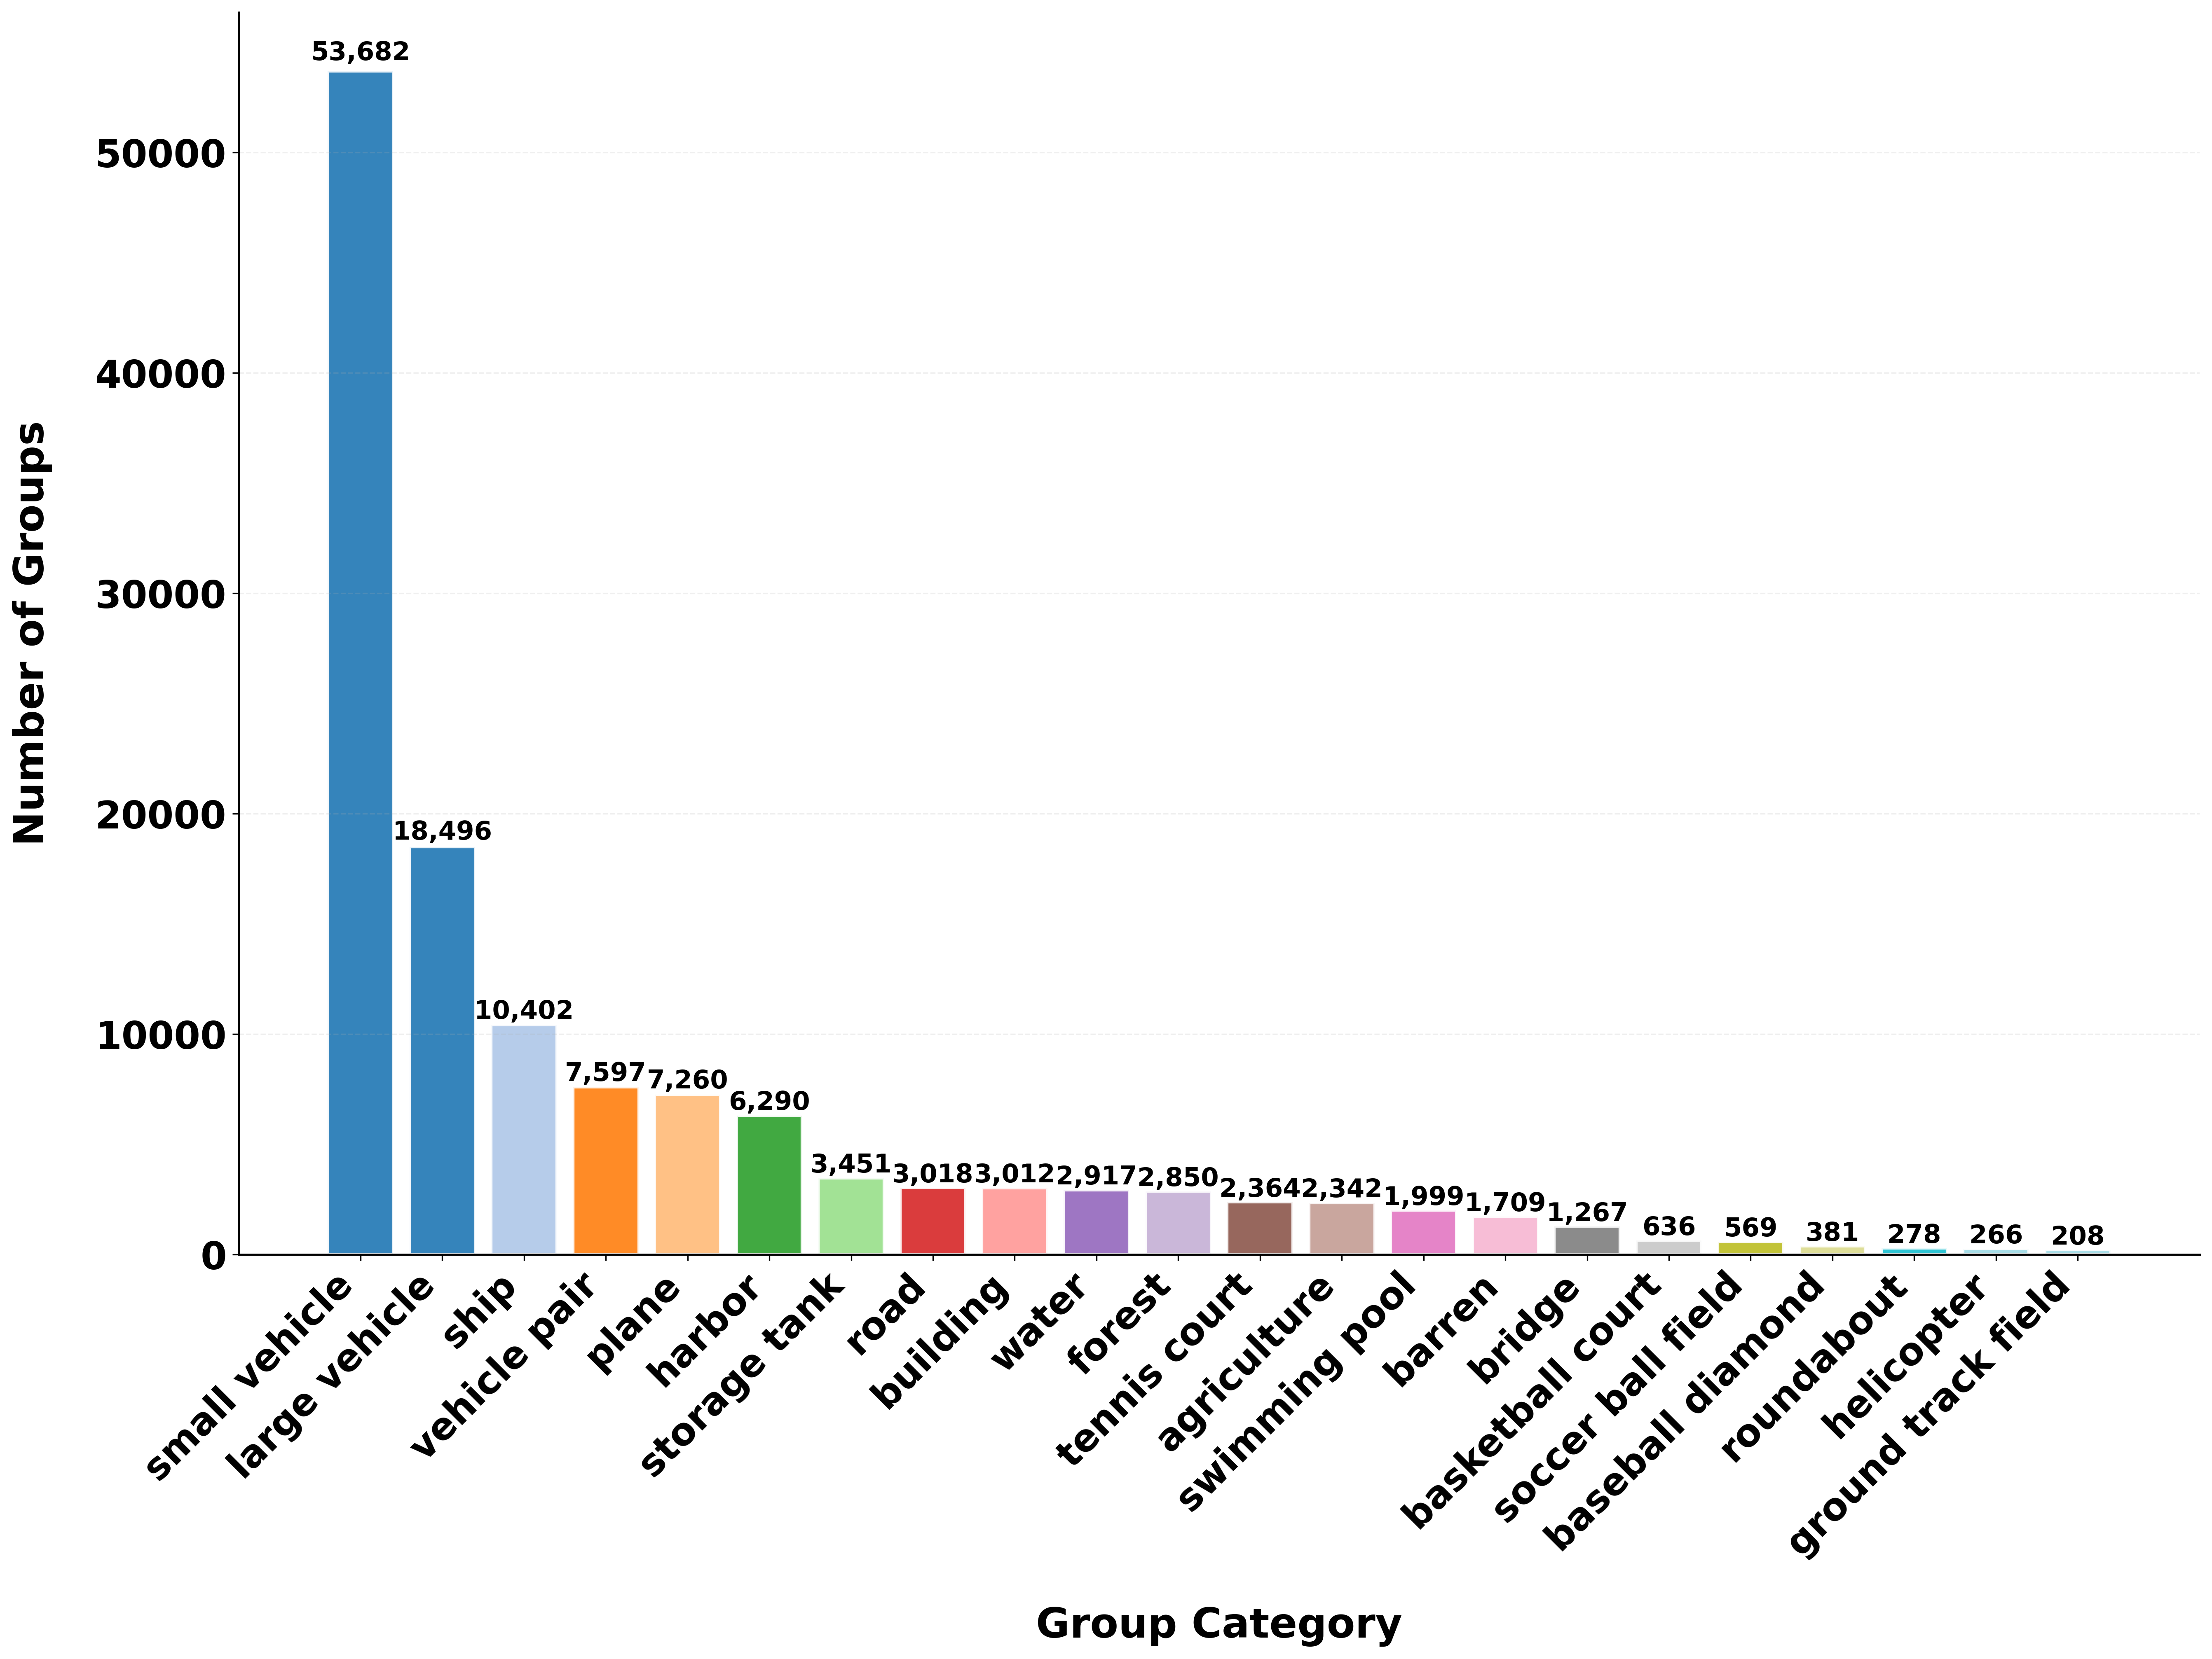
\includegraphics[width=\textwidth]{./images/group_category_distribution.png}
\end{minipage}\hfill
\begin{minipage}{0.48\textwidth}
\centering
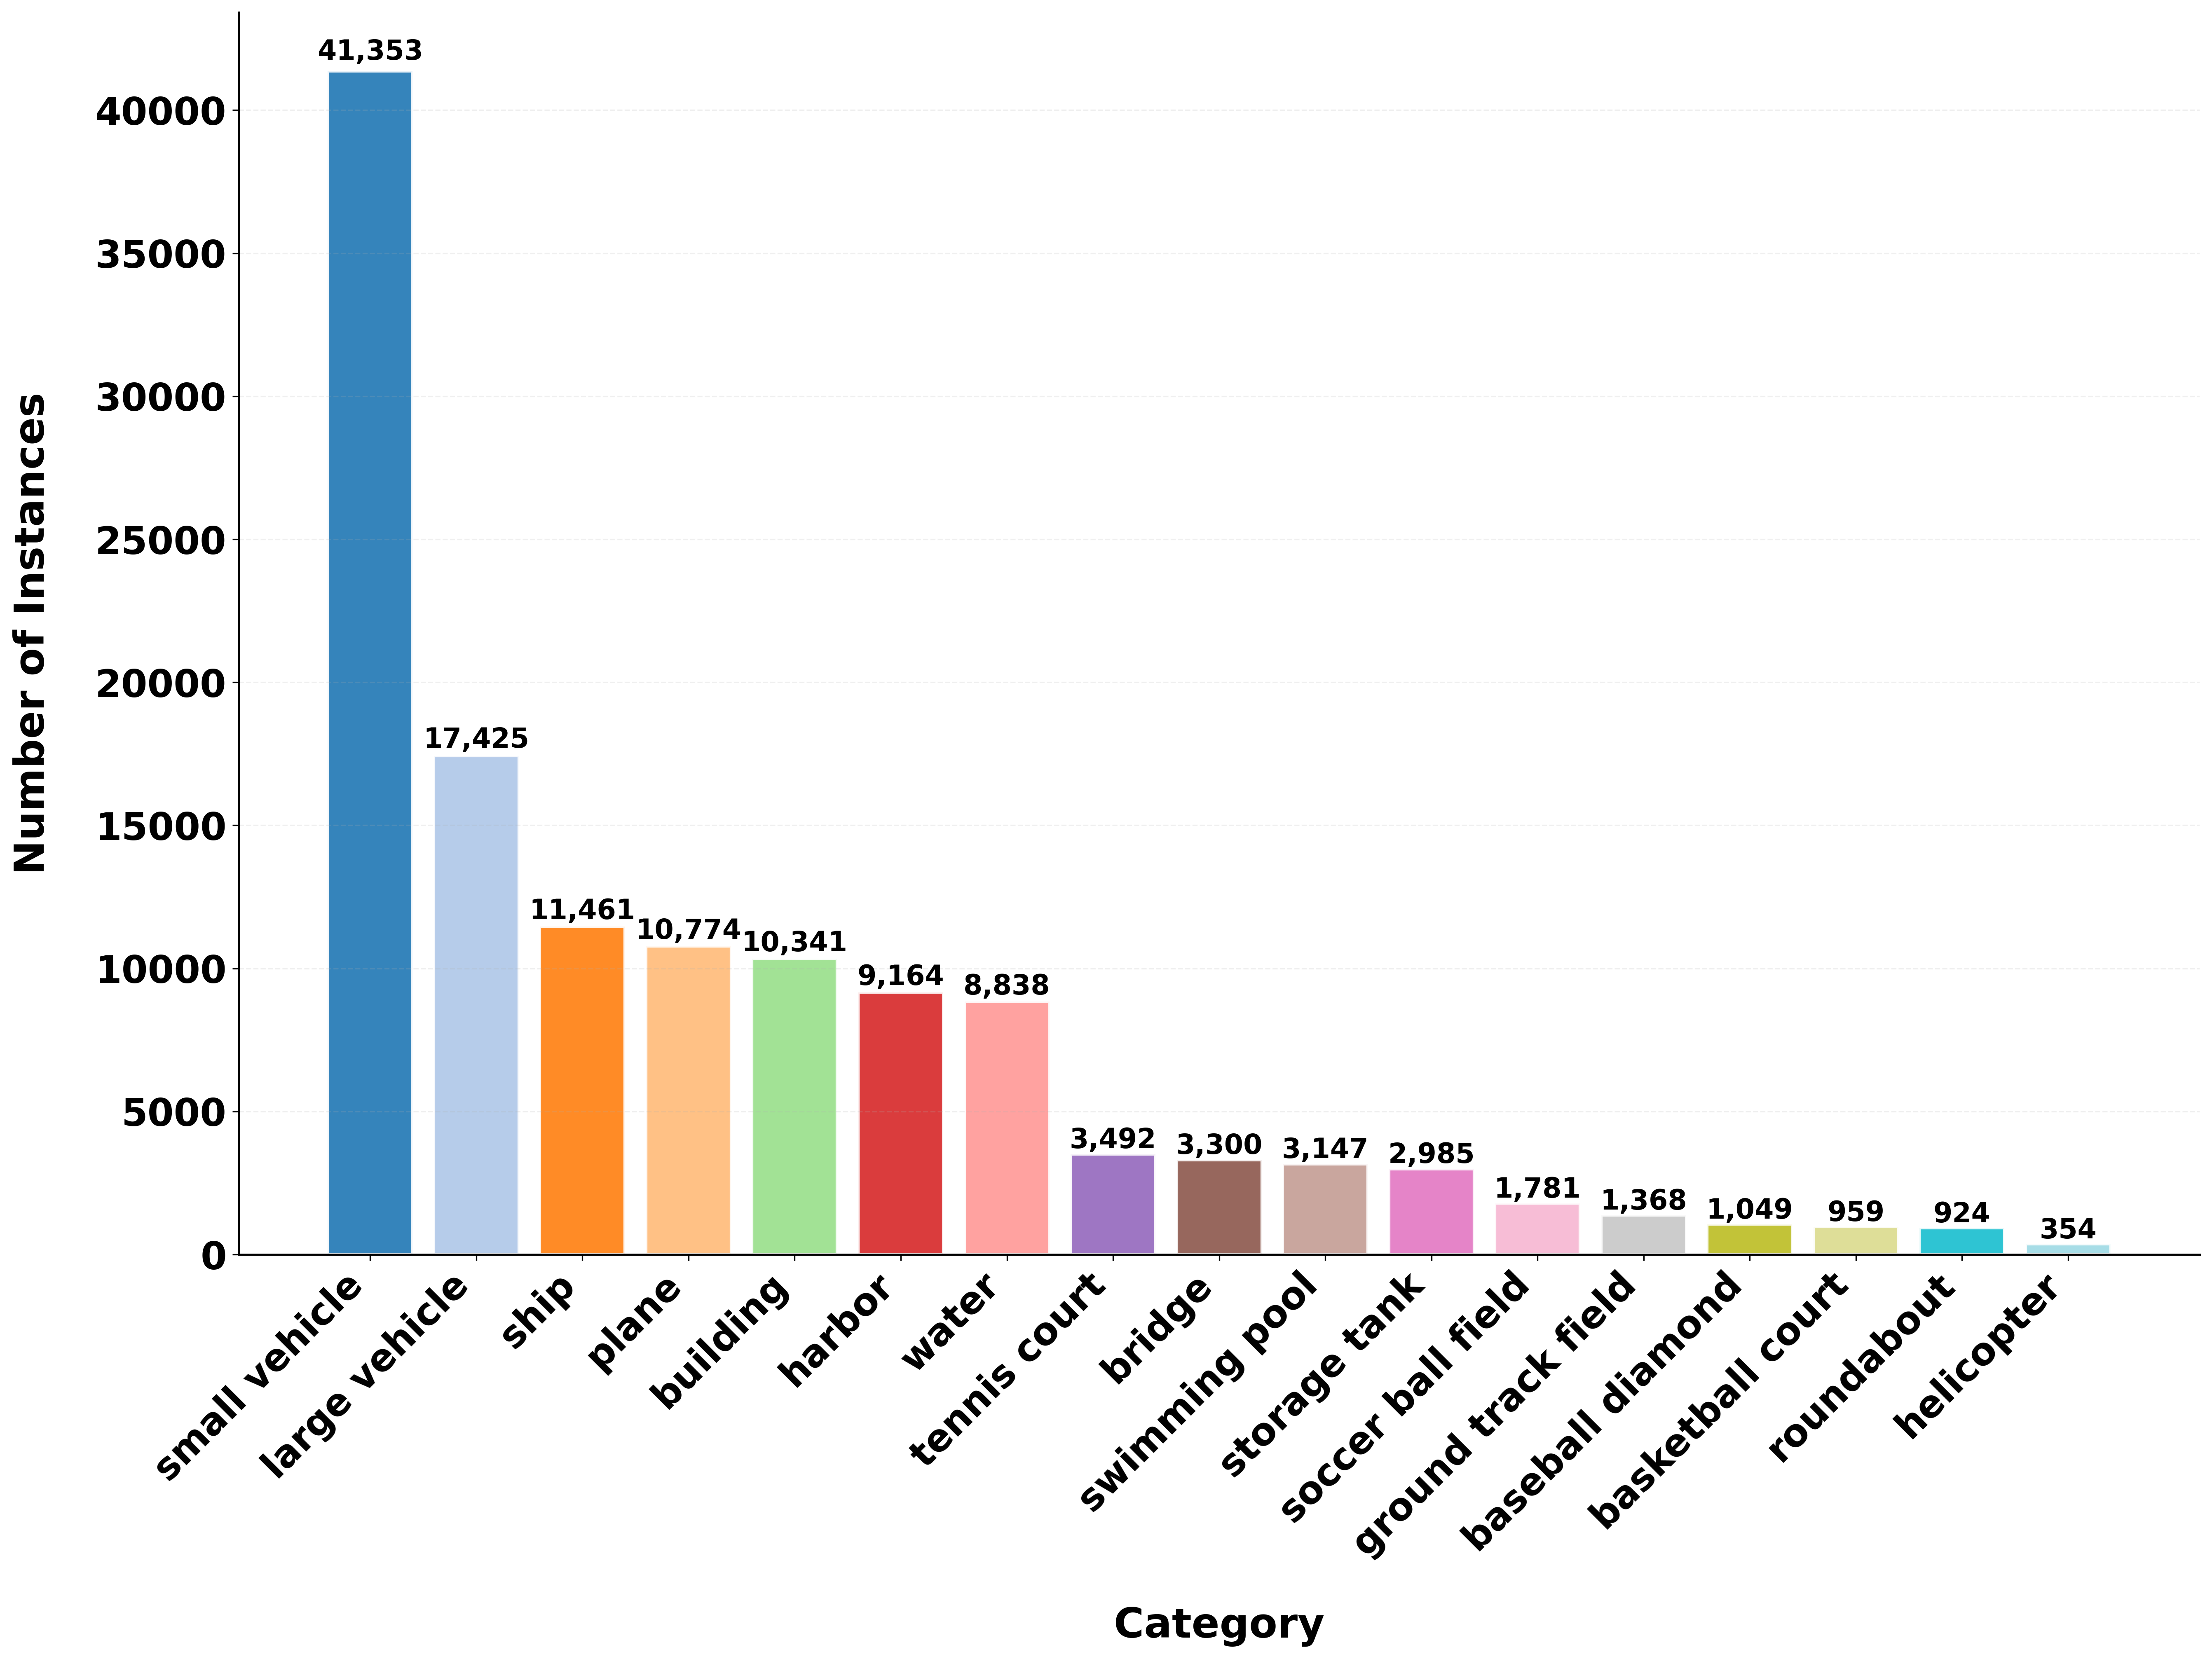
\includegraphics[width=\textwidth]{./images/instance_category_distribution.png}
\end{minipage}
\caption{Category distribution analysis of Aerial-D dataset. Left: Distribution of group annotations showing the prevalence of different object categories in group-level referring expressions. Right: Distribution of individual instance annotations across semantic categories, demonstrating the dataset's coverage of aerial object types.}
\label{fig:category_distributions}
\end{figure*}

Table \ref{tab:llm_enhancement_stats} quantifies the impact of LLM enhancement, showing that the distillation pipeline successfully tripled the dataset size from the original 506,194 rule-based expressions to 1,522,523 total expressions. The LLM enhancement process contributed nearly equal numbers of language variations (496,895) and unique visual detail expressions (519,434), demonstrating the effectiveness of the two-pronged enhancement strategy in achieving both linguistic diversity and contextual richness.

\begin{table}[H]
\centering
\caption{LLM Enhancement Expression Distribution}
\label{tab:llm_enhancement_stats}
\begin{tabular}{@{}lrrr@{}}
\toprule
\textbf{Expression Source} & \textbf{Train} & \textbf{Val} & \textbf{Total} \\
\midrule
Rule-Based Expressions & 371,360 & 134,834 & 506,194 \\
LLM Enhanced (Language Variations) & 364,396 & 132,499 & 496,895 \\
LLM Unique (Visual Details) & 382,038 & 137,396 & 519,434 \\
\midrule
\textbf{Total Expressions} & \textbf{1,117,794} & \textbf{404,729} & \textbf{1,522,523} \\
\bottomrule
\end{tabular}
\end{table}
